\documentclass[conference]{IEEEtran}
\IEEEoverridecommandlockouts

\usepackage{cite}
\usepackage{amsmath,amssymb,amsfonts}
\usepackage{graphicx}
\usepackage{textcomp}
\usepackage{xcolor}
\usepackage{booktabs}
\usepackage{array}
\usepackage{multirow}
\usepackage{hyperref}
\usepackage[utf8]{inputenc}
\usepackage[T1]{fontenc}
\graphicspath{{figs/rf/}}

\def\BibTeX{{\rm B\kern-.05em{\sc i\kern-.025em b}\kern-.08em
    T\kern-.1667em\lower.7ex\hbox{E}\kern-.125emX}}

\begin{document}

\title{Detecção de Área Queimada com Random Forest em Imagens Landsat~8 e~9:
Avaliação de Estratégias para Desbalanceamento e Validação Espacial}

\author{
  \IEEEauthorblockN{Matheus V. M. Sales}
  \IEEEauthorblockA{
    \textit{Departamento de Ciências da Computação}\\
    \textit{Universidade Federal de Pernambuco}\\
    Recife, Brasil\\
    matheusvmsales1@gmail.com
  }
}

\maketitle

%---------------------------------------------------------------------
\begin{abstract}
Este trabalho apresenta uma \textit{pipeline} completa de classificação binária
para detecção de área queimada em imagens Landsat~8 e~9, utilizando Random
Forest com validação por blocos espaciais. Dez atributos espectrais multitemporais
(bandas~B4, B5, B7, NDVI e NBR nas datas pré- e pós-incêndio) são extraídos de
duas cenas com desbalanceamento de classe de aproximadamente 20:1.
Quatro estratégias de tratamento de desbalanceamento são comparadas:
\textit{class\_weight}, \textit{undersampling}, SMOTE e SMOTETomek.
A validação por blocos espaciais em grade~$4\times4$ previne o vazamento
espacial típico de divisões aleatórias de pixels. O melhor modelo intra-cena
atinge $F_2 = 0{,}3951$ e Recall~$= 0{,}600$, enquanto a validação cruzada
entre cenas obtém $F_2 = 0{,}4715$ e Recall~$= 0{,}657$, demonstrando boa
generalização espacial. A análise de importância de atributos confirma ausência
de circularidade entre \textit{features} e rótulos, com distribuição equilibrada
de contribuições (8,3\%–11,5\% por atributo).
\end{abstract}

\begin{IEEEkeywords}
área queimada, Random Forest, Landsat, desbalanceamento de classes,
validação espacial, SMOTE, sensoriamento remoto.
\end{IEEEkeywords}

%=====================================================================
\section{Introdução}

O mapeamento de áreas queimadas é uma tarefa essencial para o monitoramento
ambiental, gestão de recursos naturais e avaliação de impactos sobre o ciclo
do carbono. No Brasil, a crescente incidência de queimadas, especialmente no
bioma Cerrado e na Amazônia, reforça a necessidade de métodos automatizados,
escaláveis e reprodutíveis para detecção em imagens de satélite de médio
resolução~\cite{b1}.

Imagens Landsat~8 e~9 oferecem revisita de aproximadamente 8~dias com resolução
espacial de 30~metros, constituindo um dos principais insumos para mapeamento
de queimadas em escala regional. Métodos baseados em limiares espectrais, como
o Índice de Área Queimada Normalizado Diferenciado (\textit{dNBR}), são amplamente
empregados por sua simplicidade operacional~\cite{b2}. Contudo, tais abordagens
dependem de calibração manual do limiar e não exploram a combinação de múltiplas
bandas espectrais disponíveis no sensor.

Algoritmos de aprendizado de máquina, em particular o Random
Forest~\cite{b3}, têm demonstrado resultados promissores em classificação de
uso e cobertura da terra. No entanto, dois desafios metodológicos recorrentes
limitam a validade dos experimentos na literatura:
(i)~o forte desbalanceamento entre pixels queimados e não queimados
($\approx1$:20); e
(ii)~a dependência espacial entre pixels vizinhos, que invalida avaliações
baseadas em divisão aleatória de amostras~\cite{b4}.

Este trabalho propõe e avalia uma pipeline completa que endereça ambos os
desafios, comparando estratégias de tratamento de desbalanceamento e adotando
validação por blocos espaciais. Uma contribuição metodológica importante é
a exclusão deliberada do \textit{dNBR} e \textit{dNDVI} como atributos de
entrada, visto que a máscara de referência foi gerada a partir de um limiar
sobre o próprio \textit{dNBR} — o que produziria circularidade entre
\textit{features} e rótulos e métricas artificialmente perfeitas.

%=====================================================================
\section{Referencial Teórico}

\subsection{Índices Espectrais para Detecção de Queimadas}

O Índice de Razão de Queima Normalizado (\textit{NBR}) é calculado a partir das
bandas do infravermelho próximo (NIR) e do infravermelho de ondas curtas (SWIR):

\begin{equation}
  \mathrm{NBR} = \frac{\rho_{\mathrm{NIR}} - \rho_{\mathrm{SWIR}}}
                      {\rho_{\mathrm{NIR}} + \rho_{\mathrm{SWIR}}}
  \label{eq:nbr}
\end{equation}

A diferença temporal (\textit{dNBR}) é obtida subtraindo o NBR pós-evento do
pré-evento. Valores elevados de \textit{dNBR} indicam redução da vegetação e
aumento de carbono na superfície, característicos de áreas queimadas.

O Índice de Vegetação por Diferença Normalizada (\textit{NDVI}) quantifica a
densidade de vegetação verde a partir das bandas Red e NIR:

\begin{equation}
  \mathrm{NDVI} = \frac{\rho_{\mathrm{NIR}} - \rho_{\mathrm{Red}}}
                       {\rho_{\mathrm{NIR}} + \rho_{\mathrm{Red}}}
  \label{eq:ndvi}
\end{equation}

\subsection{Random Forest}

Random Forest~\cite{b3} é um ensemble de árvores de decisão treinadas com
\textit{bootstrap} e seleção aleatória de subconjuntos de atributos em cada
nó. A predição é realizada por votação majoritária (classificação) ou média
(regressão). O algoritmo é naturalmente robusto a overfitting e fornece
estimativas de importância de atributos via redução média de impureza de Gini.

\subsection{Tratamento de Desbalanceamento}

Quatro estratégias são avaliadas:

\begin{itemize}
  \item \textbf{class\_weight='balanced'}: atribui pesos inversamente
        proporcionais à frequência de cada classe durante o treinamento,
        penalizando mais erros na classe minoritária.
  \item \textbf{Undersampling aleatório}: reduz a classe majoritária ao
        tamanho da minoritária, equilibrando a distribuição ao custo de
        descartar amostras.
  \item \textbf{SMOTE}~\cite{b5}: gera amostras sintéticas da classe
        minoritária por interpolação linear entre vizinhos próximos no
        espaço de atributos.
  \item \textbf{SMOTETomek}: combina SMOTE com a remoção de pares Tomek,
        eliminando amostras de fronteira ruidosas após o
        sobreamostramento.
\end{itemize}

%=====================================================================
\section{Dados e Área de Estudo}

\subsection{Imagens Landsat}

Foram utilizadas duas cenas do nível L2SP (reflectância de superfície) do
programa Landsat, cobrindo o período de agosto de 2024, correspondente à
estação seca no Brasil Central:

\begin{itemize}
  \item \textbf{Cena 221/074} — Pré: Landsat~9 (20/08/2024);
        Pós: Landsat~8 (28/08/2024).
  \item \textbf{Cena 220/075} — Pré: Landsat~8 (21/08/2024);
        Pós: Landsat~9 (29/08/2024).
\end{itemize}

As imagens apresentam dimensões de aproximadamente $7800 \times 7700$~pixels
($\approx 40$ milhões de pixels válidos por cena após mascaramento de nuvens
e bordas). A Fig.~\ref{fig:cenas} mostra as composições falsa-cor, dNBR e
máscaras de referência para as duas cenas.

\begin{figure}[!t]
  \centering
  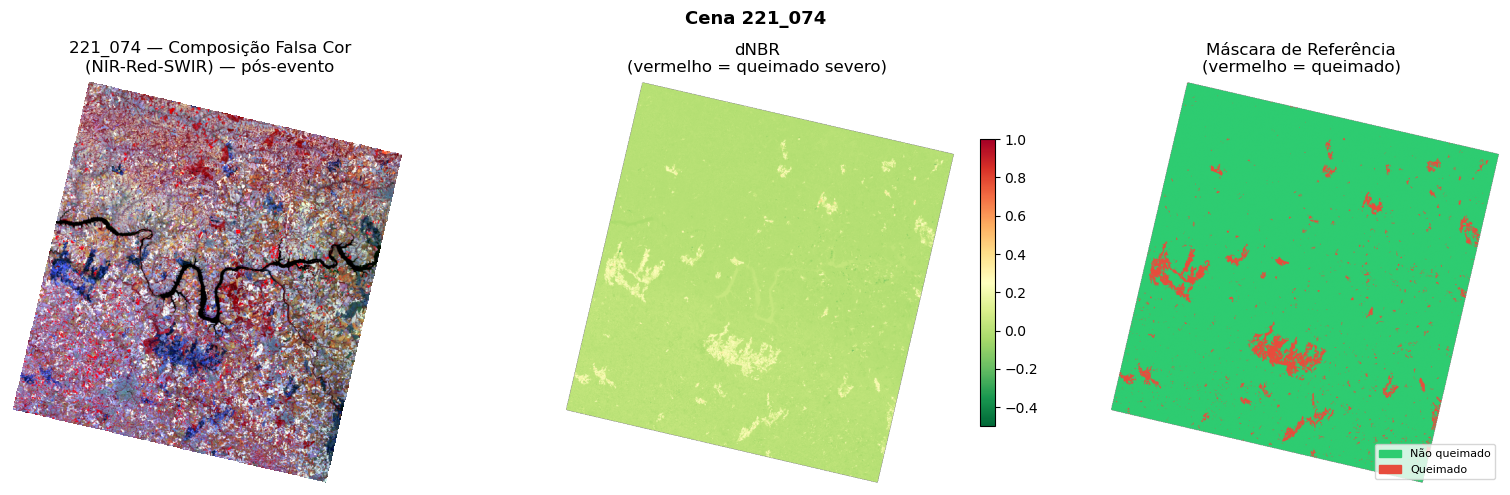
\includegraphics[width=\columnwidth]{fig_cena_221074.png}\\[3pt]
  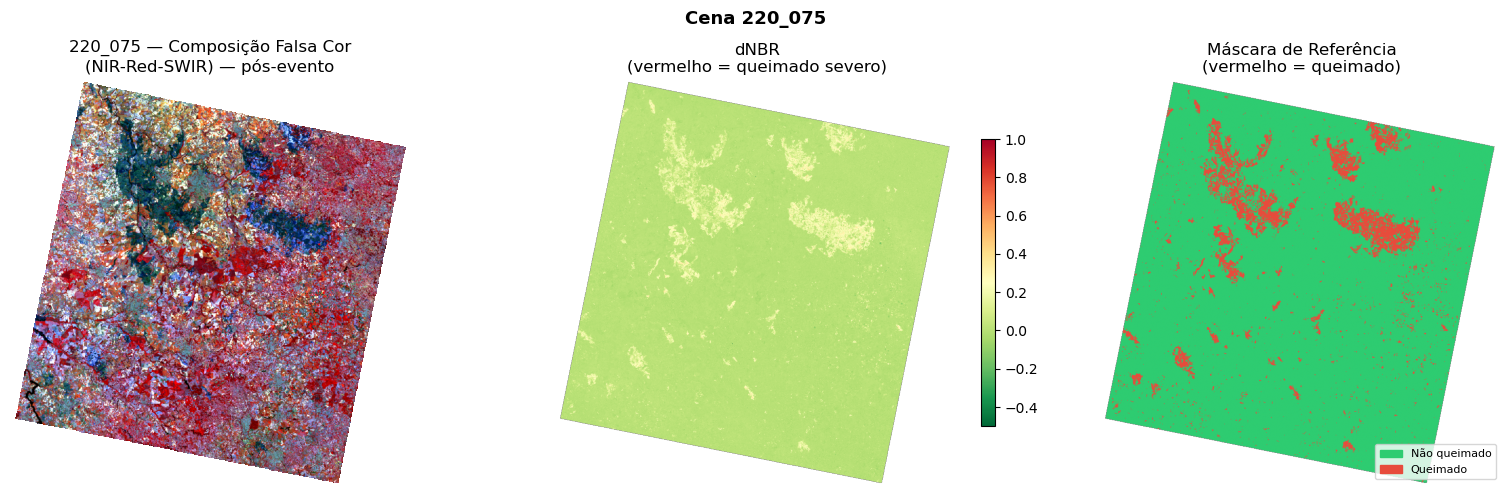
\includegraphics[width=\columnwidth]{fig_cena_220075.png}
  \caption{Composição falsa-cor NIR-Red-SWIR (esq.), dNBR (centro) e
           máscara de referência (dir.) para as cenas 221/074 (cima)
           e 220/075 (baixo). Vermelho indica área queimada.}
  \label{fig:cenas}
\end{figure}

\subsection{Atributos de Entrada}

Para cada pixel, são extraídos 10~atributos multitemporais, organizados em
três grupos:

\begin{itemize}
  \item \textbf{Pré-evento} (5): B4~(Red), B5~(NIR), B7~(SWIR2), NDVI, NBR.
  \item \textbf{Pós-evento} (5): B4, B5, B7, NDVI, NBR.
\end{itemize}

Os índices \textit{dNBR} e \textit{dNDVI} foram explicitamente excluídos do
vetor de atributos. A máscara de referência foi gerada com limiar
$\mathrm{dNBR} > 0{,}65$, portanto incluir o \textit{dNBR} como feature
criaria circularidade direta entre atributo e rótulo, produzindo métricas
artificialmente perfeitas ($F_2 = 1{,}0$, Kappa $= 1{,}0$).

\subsection{Rótulos e Desbalanceamento}

A Fig.~\ref{fig:features} ilustra as distribuições espectrais de cada atributo
por classe. A Tabela~\ref{tab:imbalance} resume a distribuição de classes nas
amostras extraídas ($n=150.000$ por cena, por subamostragem estratificada
proporcional).

\begin{figure}[!t]
  \centering
  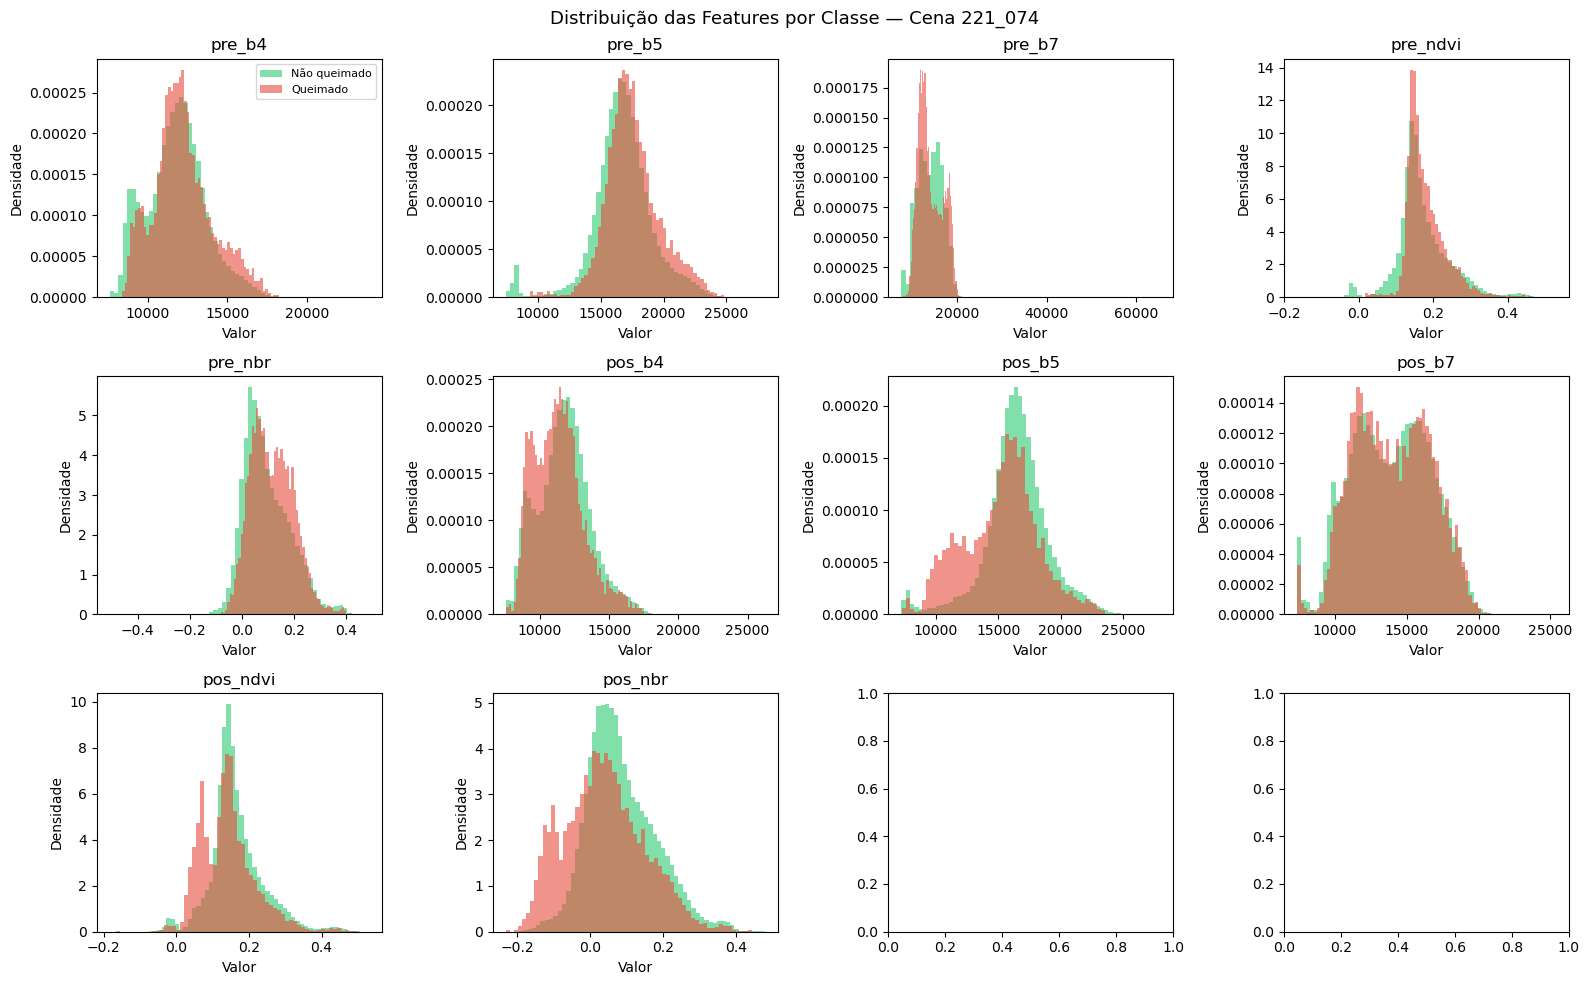
\includegraphics[width=\columnwidth]{fig_features_dist.png}
  \caption{Distribuição de densidade dos 10~atributos por classe (verde =
           não queimado; vermelho = queimado) — Cena 221/074. As bandas pré-evento
           apresentam separação bimodal mais nítida que as pós-evento isoladas.}
  \label{fig:features}
\end{figure}

\begin{table}[!t]
  \caption{Distribuição de classes nas amostras ($n = 150.000$)}
  \label{tab:imbalance}
  \centering
  \begin{tabular}{lrrr}
    \toprule
    \textbf{Cena} & \textbf{Queimado} & \textbf{Não queimado} & \textbf{Razão} \\
    \midrule
    221/074 & 7.210 (4,8\%)  & 142.790 (95,2\%) & 1:19,8 \\
    220/075 & 11.888 (7,9\%) & 138.112 (92,1\%) & 1:11,6 \\
    \bottomrule
  \end{tabular}
\end{table}

%=====================================================================
\section{Metodologia}

\subsection{Pipeline de Processamento}

A Fig.~\ref{fig:pipeline} ilustra o fluxo completo de processamento.
As etapas são:

\begin{enumerate}
  \item \textbf{Carregamento e alinhamento}: leitura das bandas GeoTIFF via
        \texttt{rasterio}, cálculo da \textit{shape} mínima comum entre todos
        os arquivos de uma cena para garantir alinhamento espacial perfeito.
  \item \textbf{Mascaramento de validade}: pixels são excluídos se qualquer
        banda apresentar valor \textit{nodata} (bandas uint16: valor~0;
        bandas float: $-3{,}4 \times 10^{38}$), ou se o rótulo não for
        estritamente 0~ou~1.
  \item \textbf{Subamostragem estratificada}: seleção de 150.000~pixels
        mantendo a proporção original de classes, viabilizando o treinamento
        sem perda de representatividade.
  \item \textbf{Validação por blocos espaciais}: divisão em grade $4 \times 4$
        (16~blocos), com 4~blocos ($\approx25\%$) sorteados para teste.
        Pixels do mesmo bloco geográfico ficam no mesmo conjunto,
        eliminando dependência espacial entre treino e teste.
  \item \textbf{Tratamento de desbalanceamento}: aplicação de uma das quatro
        estratégias ao conjunto de treino.
  \item \textbf{Treinamento e otimização}: RandomizedSearchCV com 30
        iterações e validação cruzada estratificada 5-\textit{fold} sobre o
        conjunto de treino.
  \item \textbf{Ajuste de threshold}: otimização do limiar de decisão via
        curva Precision-Recall, maximizando $F_\beta$ com $\beta=2$
        (recall ponderado duas vezes mais que precision).
  \item \textbf{Avaliação}: métricas $F_2$, MCC, Kappa, $F_1$, Precision,
        Recall e AUPRC no conjunto de teste.
  \item \textbf{Validação cruzada entre cenas}: treinamento em 221/074,
        teste em 220/075 para avaliação de generalização espacial.
  \item \textbf{Geração do mapa}: predição em batches de 100.000~pixels
        sobre a cena completa.
\end{enumerate}

\begin{figure}[!t]
  \centering
  \fbox{%
    \parbox{0.92\columnwidth}{%
      \small
      \textbf{Entrada}: GeoTIFFs Landsat (B4, B5, B7, NDVI, NBR — pré e pós)\\[2pt]
      $\downarrow$ \textit{Alinhamento e mascaramento de nodata}\\[2pt]
      $\downarrow$ \textit{Subamostragem estratificada} ($n=150\,000$)\\[2pt]
      $\downarrow$ \textit{Divisão por blocos espaciais} ($4\times4$, 75/25)\\[2pt]
      $\downarrow$ \textit{Tratamento de desbalanceamento}
                   (undersampling / SMOTE / pesos)\\[2pt]
      $\downarrow$ \textit{Treinamento RF + RandomizedSearchCV}\\[2pt]
      $\downarrow$ \textit{Otimização de threshold via curva PR ($F_2$)}\\[2pt]
      $\downarrow$ \textit{Avaliação intra-cena e cross-cena}\\[2pt]
      \textbf{Saída}: Mapa binário de área queimada + métricas
    }%
  }
  \caption{Pipeline de detecção de área queimada.}
  \label{fig:pipeline}
\end{figure}

\subsection{Validação por Blocos Espaciais}

A dependência espacial entre pixels vizinhos é o principal fator que invalida
avaliações com divisão aleatória: pixels de treino e teste podem ser
geograficamente adjacentes, inflando artificialmente as métricas por
autocorrelação espacial~\cite{b4}.

Neste trabalho, cada pixel $(r,c)$ é atribuído ao bloco
$b = \lfloor r/H \cdot k \rfloor \cdot k + \lfloor c/W \cdot k \rfloor$,
onde $k=4$ é o número de blocos por lado e $(H,W)$ é o tamanho da cena.
Quatro blocos são sorteados para o conjunto de teste, garantindo separação
geográfica mínima de $\approx 1{,}9~\mathrm{km}$ entre fronteiras de bloco.
A Fig.~\ref{fig:blocos} ilustra a divisão aplicada à cena~221/074.

\begin{figure}[!t]
  \centering
  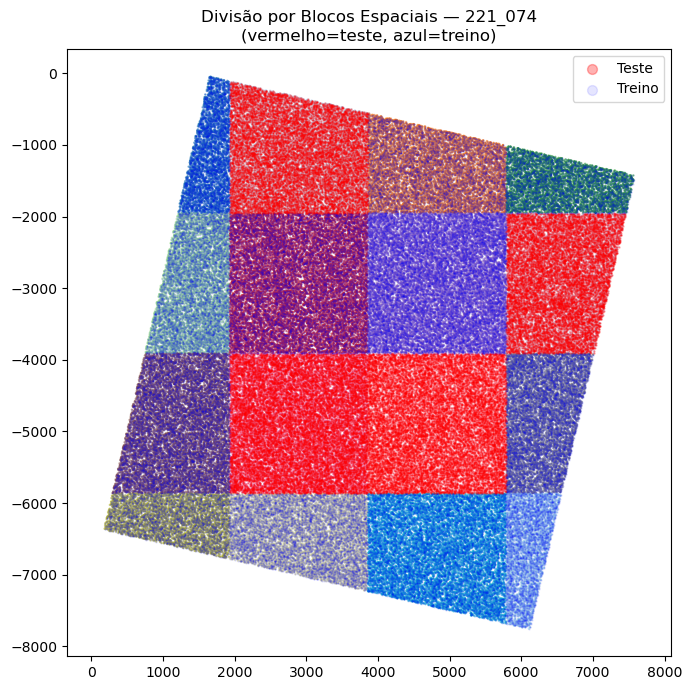
\includegraphics[width=0.85\columnwidth]{fig_blocos_espaciais.png}
  \caption{Divisão por blocos espaciais ($4\times4$, 16~blocos) na cena 221/074.
           Pixels em vermelho pertencem ao conjunto de teste (blocos~1, 7, 9, 10);
           azul indica treino. A separação geográfica evita autocorrelação
           espacial entre conjuntos.}
  \label{fig:blocos}
\end{figure}

\subsection{Ajuste de Threshold}

O threshold padrão $p=0{,}5$ é inadequado para dados desbalanceados:
o modelo tende a raramente atribuir $p>0{,}5$ à classe minoritária.
Para cada modelo, varre-se o intervalo $[0,1]$ sobre a curva
Precision-Recall e seleciona-se o threshold $\tau^*$ que maximiza
$F_2$:

\begin{equation}
  \tau^* = \underset{\tau}{\arg\max}\;
  F_2(\tau) = \frac{5 \cdot P(\tau) \cdot R(\tau)}
                   {4 \cdot P(\tau) + R(\tau)}
  \label{eq:f2}
\end{equation}

\subsection{Métricas de Avaliação}

Além de $F_2$ e acurácia global (OA), reportamos:

\begin{itemize}
  \item \textbf{MCC} (\textit{Matthews Correlation Coefficient}): métrica
        balanceada robusta a desbalanceamento, no intervalo $[-1, 1]$.
  \item \textbf{Kappa de Cohen}: concordância acima do acaso, descontando
        a acurácia esperada aleatoriamente.
  \item \textbf{AUPRC} (\textit{Area Under Precision-Recall Curve}):
        síntese do desempenho em todos os thresholds possíveis.
\end{itemize}

%=====================================================================
\section{Experimentos e Resultados}

\subsection{Comparação das Estratégias de Desbalanceamento}

A Tabela~\ref{tab:estrategias} apresenta os resultados das quatro estratégias
no conjunto de teste da cena~221/074 (blocos espaciais).

\begin{table}[!t]
  \caption{Comparação de estratégias de desbalanceamento — Cena 221/074}
  \label{tab:estrategias}
  \centering
  \setlength{\tabcolsep}{4pt}
  \begin{tabular}{lcccccc}
    \toprule
    \textbf{Estratégia} & \textbf{$F_2$} & \textbf{MCC} & \textbf{Kappa}
                        & \textbf{Prec.} & \textbf{Recall} & \textbf{AUPRC} \\
    \midrule
    Sem tratamento          & 0,021 & 0,088 & 0,030 & 0,535 & 0,017 & 0,202 \\
    \textit{class\_weight}  & 0,017 & 0,086 & 0,024 & 0,632 & 0,013 & 0,191 \\
    SMOTE                   & 0,234 & 0,173 & 0,172 & 0,200 & 0,245 & 0,154 \\
    SMOTETomek              & 0,235 & 0,173 & 0,172 & 0,200 & 0,245 & 0,158 \\
    Undersampling           & \textbf{0,354} & \textbf{0,198} & 0,122
                            & 0,117 & \textbf{0,716} & 0,216 \\
    \textit{class\_weight} + $\tau^*$  & 0,346 & 0,198 & 0,151 & 0,140 & 0,547 & 0,191 \\
    \bottomrule
  \end{tabular}
\end{table}

O baseline sem tratamento apresenta Recall de apenas 1,7\%, confirmando que
o Random Forest ignora a classe minoritária sem intervenção. O
\textit{class\_weight='balanced'} com threshold padrão tem desempenho ainda
inferior, pois produz distribuições de probabilidade mais difusas que
requerem redução do threshold. Com $\tau^* = 0{,}07$, o mesmo modelo
alcança $F_2 = 0{,}346$ e Recall~$= 0{,}547$.

\begin{figure}[!t]
  \centering
  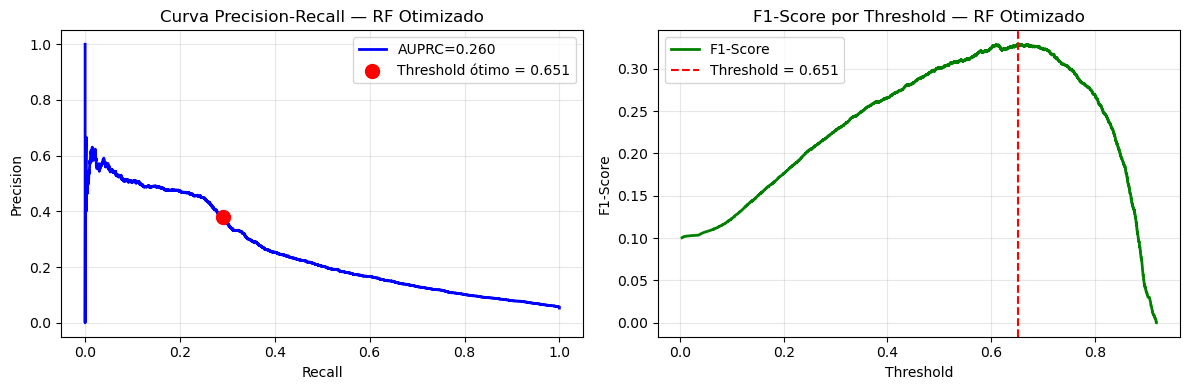
\includegraphics[width=\columnwidth]{fig_threshold_pr.png}
  \caption{Curva Precision-Recall e $F_2$ por threshold para o modelo
           \textit{class\_weight='balanced'}: $\tau^* = 0{,}07$ maximiza
           $F_2$ (AUPRC~$= 0{,}191$).}
  \label{fig:threshold_pr}
\end{figure}

O Undersampling obtém o maior Recall (71,6\%) ao custo de Precision baixa
(11,7\%), característica esperada do forte balanceamento por descarte.
SMOTE e SMOTETomek produzem resultados similares entre si ($F_2 \approx 0{,}234$),
com desempenho inferior ao Undersampling — possivelmente porque amostras
sintéticas geradas por interpolação linear em regiões de fronteira
espectral introduzem ruído nos limites de decisão.
A Fig.~\ref{fig:estrategias} compara visualmente as métricas.

\begin{figure}[!t]
  \centering
  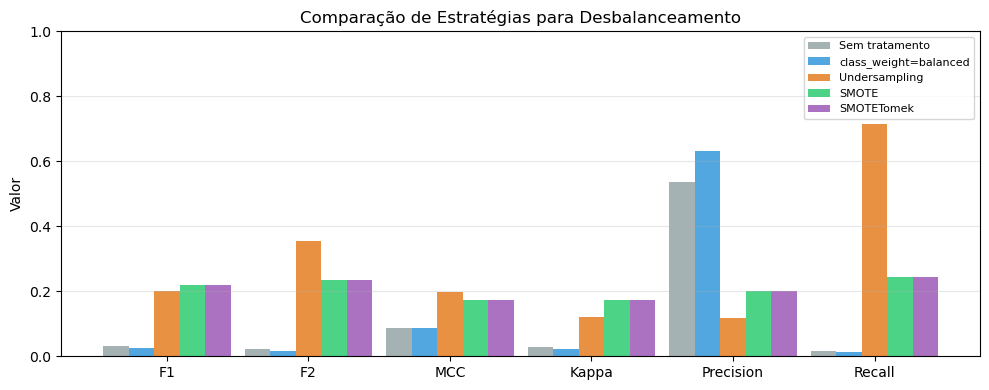
\includegraphics[width=\columnwidth]{fig_estrategias_comp.png}
  \caption{Comparação das estratégias de desbalanceamento por métrica de
           avaliação ($F_2$, MCC, Kappa, $F_1$, Precision, Recall).
           Undersampling lidera em $F_2$ e Recall com threshold padrão.}
  \label{fig:estrategias}
\end{figure}

\begin{figure}[!t]
  \centering
  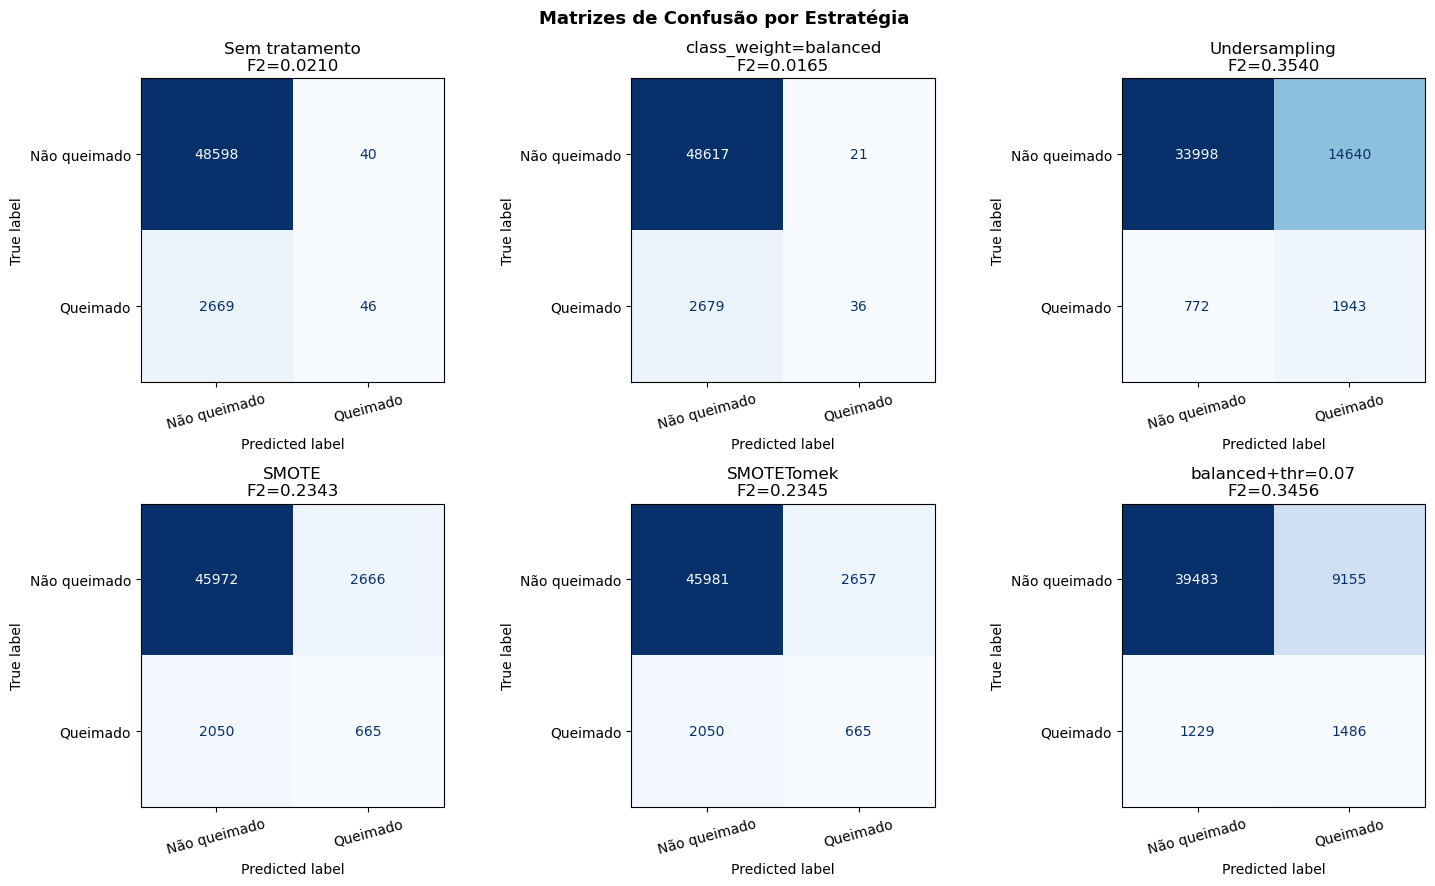
\includegraphics[width=\columnwidth]{fig_conf_matrices.png}
  \caption{Matrizes de confusão normalizadas para cada estratégia de
           desbalanceamento — cena~221/074. Undersampling maximiza o Recall
           (células TP mais escuras) ao custo de maior taxa de FP.}
  \label{fig:conf_matrices}
\end{figure}

\subsection{Otimização de Hiperparâmetros}

A busca por RandomizedSearchCV (30~iterações, 5-\textit{fold} CV,
critério~$F_1$) sobre o conjunto de treino da cena~221/074 retornou os
seguintes hiperparâmetros ótimos:

\begin{itemize}
  \item \texttt{class\_weight}: \texttt{balanced}
  \item \texttt{max\_depth}: 30
  \item \texttt{max\_features}: \texttt{sqrt}
  \item \texttt{min\_samples\_leaf}: 11
  \item \texttt{min\_impurity\_decrease}: $10^{-4}$
  \item \texttt{n\_estimators}: 171
\end{itemize}

O valor \texttt{min\_samples\_leaf=11} e \texttt{min\_impurity\_decrease=$10^{-4}$}
indicam que a busca encontrou um nível de regularização relevante: folhas
com menos de 11 amostras ou ganho muito pequeno não são criadas, evitando
o overfitting a ruídos espectrais pontuais. O melhor $F_1$ em
validação cruzada foi $0{,}2211$.

\subsection{Modelo Otimizado e Ajuste de Threshold}

A Tabela~\ref{tab:otimizado} compara o modelo otimizado com e sem ajuste de
threshold.

\begin{table}[!t]
  \caption{Modelo otimizado — efeito do ajuste de threshold}
  \label{tab:otimizado}
  \centering
  \begin{tabular}{lcccccc}
    \toprule
    \textbf{Configuração} & \textbf{$F_2$} & \textbf{MCC} & \textbf{Kappa}
                          & \textbf{Prec.} & \textbf{Recall} & $\tau$ \\
    \midrule
    RF Otimizado $\tau=0{,}5$  & 0,379 & 0,267 & 0,248 & 0,224 & 0,459 & 0,50 \\
    RF Otimizado $\tau^*$      & \textbf{0,395} & 0,247 & 0,194 & 0,167 & 0,601 & 0,38 \\
    \bottomrule
  \end{tabular}
\end{table}

O ajuste do threshold de $0{,}5$ para $\tau^* = 0{,}378$ eleva o Recall de
45,9\% para 60,1\% ($+14{,}2$~p.p.) com redução moderada da Precision
(22,4\% → 16,7\%). O ganho em $F_2$ é de $+0{,}016$, refletindo que
a métrica privilegia o Recall. A Fig.~\ref{fig:threshold} mostra as curvas
Precision-Recall e $F_2$ por threshold para o modelo otimizado.

\begin{figure}[!t]
  \centering
  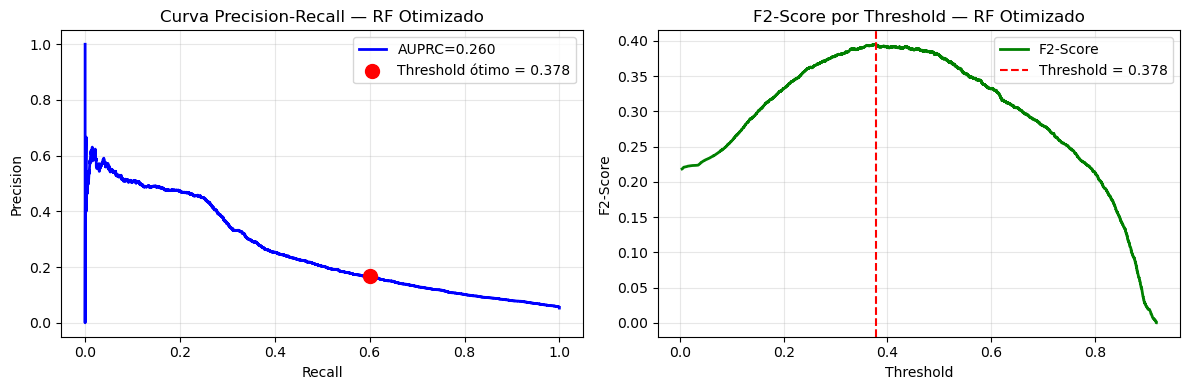
\includegraphics[width=\columnwidth]{fig_threshold_otimizado.png}
  \caption{Modelo otimizado: curva Precision-Recall com AUPRC e ponto
           ótimo (esq.); $F_2$-score por threshold com $\tau^* = 0{,}378$
           assinalado (dir.).}
  \label{fig:threshold}
\end{figure}

\subsection{Validação Cruzada Entre Cenas}

O modelo otimizado treinado na cena completa 221/074 ($n=150.000$) foi
avaliado diretamente na cena 220/075, sem re-treinamento. Os resultados
são apresentados na Tabela~\ref{tab:crosscena}.

\begin{table}[!t]
  \caption{Validação cruzada entre cenas}
  \label{tab:crosscena}
  \centering
  \begin{tabular}{lcccccc}
    \toprule
    \textbf{Treino → Teste} & \textbf{$F_2$} & \textbf{MCC} & \textbf{Kappa}
                            & \textbf{Prec.} & \textbf{Recall} & \textbf{AUPRC} \\
    \midrule
    221/074 → Intra  & 0,395 & 0,247 & 0,194 & 0,167 & 0,601 & 0,260 \\
    221/074 → 220/075 & \textbf{0,472} & \textbf{0,292} & \textbf{0,241}
                      & 0,222 & \textbf{0,657} & \textbf{0,467} \\
    \bottomrule
  \end{tabular}
\end{table}

O modelo generaliza bem para a cena não vista: $F_2 = 0{,}472$
($+0{,}077$ sobre a validação intra-cena) e AUPRC~$= 0{,}467$
($+0{,}207$). Dois fatores contribuem para esse resultado:
(i)~a cena~220/075 possui maior proporção de queimado (7,9\% vs.\ 4,8\%),
reduzindo o desbalanceamento efetivo durante o teste; e
(ii)~o treinamento com a cena~221/074 completa provê mais exemplos
positivos do que os 75\% dos blocos de treino na validação intra-cena.

\subsection{Importância de Atributos}

A distribuição de importância (redução média de impureza de Gini) no modelo
otimizado é apresentada na Tabela~\ref{tab:importancia}.

\begin{table}[!t]
  \caption{Importância dos atributos — modelo otimizado (\textit{class\_weight=balanced})}
  \label{tab:importancia}
  \centering
  \begin{tabular}{clc}
    \toprule
    \textbf{Rank} & \textbf{Atributo} & \textbf{Importância} \\
    \midrule
    1  & pre\_ndvi & 0,1145 (11,5\%) \\
    2  & pre\_b4   & 0,1106 (11,1\%) \\
    3  & pre\_nbr  & 0,1094 (10,9\%) \\
    4  & pos\_nbr  & 0,1091 (10,9\%) \\
    5  & pre\_b7   & 0,1061 (10,6\%) \\
    6  & pos\_b5   & 0,0985 (9,9\%)  \\
    7  & pre\_b5   & 0,0956 (9,6\%)  \\
    8  & pos\_ndvi & 0,0899 (9,0\%)  \\
    9  & pos\_b7   & 0,0835 (8,4\%)  \\
    10 & pos\_b4   & 0,0828 (8,3\%)  \\
    \midrule
    — & \textbf{Top 2 somam} & \textbf{22,5\%} \\
    \bottomrule
  \end{tabular}
\end{table}

\begin{figure}[!t]
  \centering
  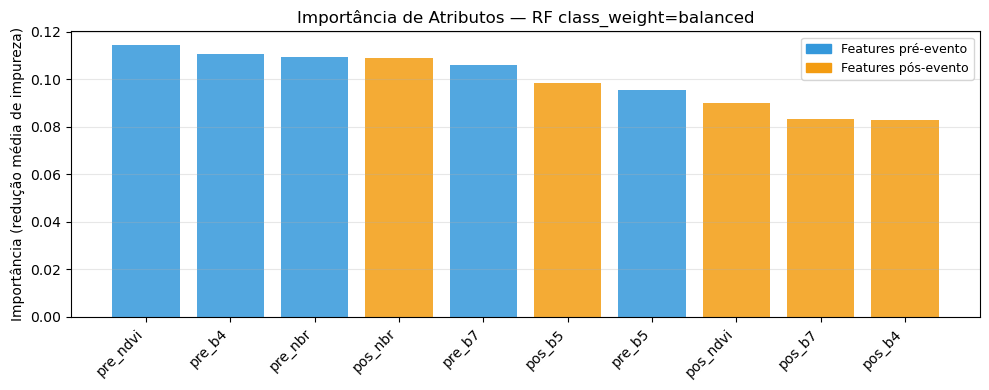
\includegraphics[width=\columnwidth]{fig_importancia.png}
  \caption{Importância de atributos (redução média de impureza de Gini) —
           modelo otimizado. Azul = features pré-evento; laranja = features
           pós-evento. Distribuição uniforme confirma ausência de leakagem.}
  \label{fig:importancia}
\end{figure}

A distribuição é notavelmente uniforme (amplitude de apenas 3,2~p.p. entre
o atributo mais e menos importante), contrastando com o cenário anterior à
correção de leakagem, em que \textit{dnbr} + \textit{dndvi} respondiam por
95,6\% da importância total. A ausência de dominância de atributo único
confirma que o modelo agora aprende relações multiespectrais genuínas.

Os atributos pré-evento (NDVI, B4, NBR) lideram marginalmente, sugerindo
que o estado da vegetação antes do incêndio é mais discriminativo que o
estado pós-evento isolado — provavelmente porque áreas com vegetação
densa pré-evento apresentam contraste espectral mais acentuado após a queima.

\subsection{Mapa de Predição na Imagem Completa}

O modelo otimizado foi aplicado a 1,5~milhão de pixels da cena~221/074
completa. A Tabela~\ref{tab:mapa} resume os resultados pixel a pixel.

\begin{table}[!t]
  \caption{Métricas do mapa de predição completo — Cena 221/074}
  \label{tab:mapa}
  \centering
  \begin{tabular}{lrr}
    \toprule
    \textbf{Classe predita} & \textbf{Ref.\ Queimado} & \textbf{Ref.\ Não queimado} \\
    \midrule
    Predito Queimado     & TP = 1.467 & FP = 10.307 \\
    Predito Não queimado & FN = 1.405 & TN = 47.271 \\
    \midrule
    \textbf{Precision}  & \multicolumn{2}{c}{12,46\%} \\
    \textbf{Recall}     & \multicolumn{2}{c}{51,08\%} \\
    \textbf{$F_2$}      & \multicolumn{2}{c}{0,3153}  \\
    \textbf{\% pred. queimado} & \multicolumn{2}{c}{19,5\% (real: 4,8\%)} \\
    \bottomrule
  \end{tabular}
\end{table}

A queda de $F_2$ de $0{,}395$ (validação) para $0{,}315$ (mapa completo)
é esperada e indica ausência de super-otimismo: o modelo não estava
memorizando os blocos de teste. A proporção de área predita como queimada
(19,5\% vs.\ 4,8\% real) revela a presença de falsos positivos,
concentrados provavelmente em solos expostos, corpos d'água escuros e
sombras de nuvem — feições que compartilham assinatura espectral com
área queimada.

\subsection{Ranking Final das Estratégias}

A Fig.~\ref{fig:ranking_final} consolida todas as estratégias em um ranking
por métrica, permitindo a escolha da abordagem mais adequada ao objetivo da
aplicação.

\begin{figure}[!t]
  \centering
  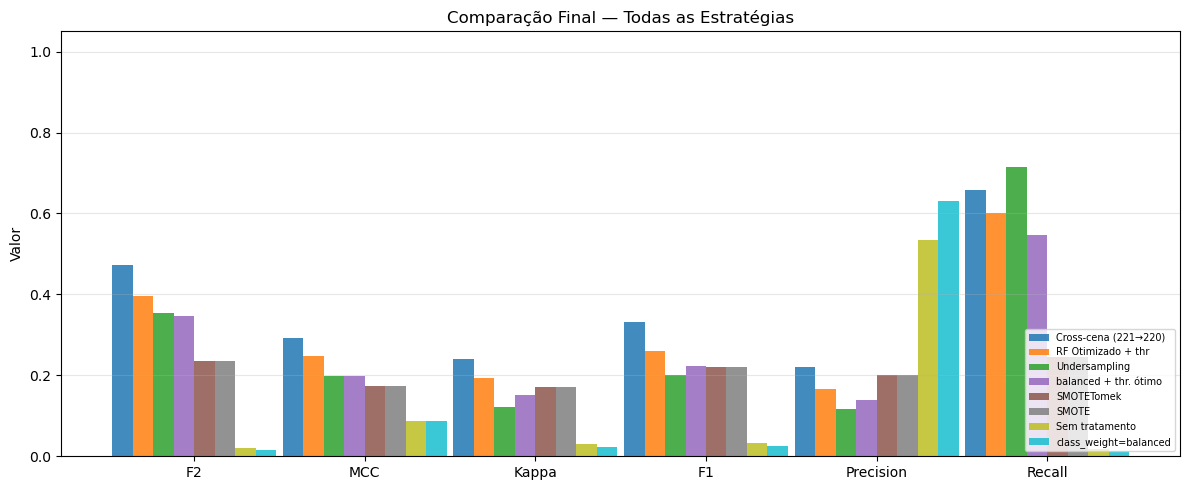
\includegraphics[width=\columnwidth]{fig_ranking_final.png}
  \caption{Ranking final das estratégias por métrica ($F_2$, Recall, MCC,
           Kappa, AUPRC). Undersampling lidera em $F_2$ e Recall;
           \textit{class\_weight} com $\tau^*$ equilibra melhor Precision
           e Kappa.}
  \label{fig:ranking_final}
\end{figure}

%=====================================================================
\section{Discussão}

\subsection{Impacto do Leakagem na Validação}

A principal contribuição metodológica deste trabalho é a demonstração
explícita do impacto da circularidade entre atributos e rótulos.
Quando \textit{dNBR} e \textit{dNDVI} eram incluídos como \textit{features},
todas as estratégias (exceto Undersampling) atingiam $F_2 = 1{,}0000$ e
Kappa~$= 1{,}0000$, independentemente da validação por blocos espaciais.
A importância de atributos revelava o problema: dois atributos respondiam
por 95,6\% da importância total.

Após a remoção, os valores caíram para intervalos realistas
($F_2 \in [0{,}02,\, 0{,}47]$), as estratégias de balanceamento passaram
a mostrar diferenças reais, e a importância distribuiu-se uniformemente
entre os 10 atributos restantes. Esse resultado alerta para um risco
recorrente em trabalhos de mapeamento remoto: utilizar como feature o
mesmo índice espectral que gerou a máscara de referência.

\subsection{Limitações do Modelo Sem Índices de Diferença}

A exclusão de \textit{dNBR} e \textit{dNDVI} é necessária para a validade
metodológica com a máscara atual, mas representa uma perda de informação
físicamente relevante: a variação temporal entre pré e pós-evento é o
sinal mais discriminativo para queimadas. O modelo passa a diferenciar
queimado de não-queimado exclusivamente pelo estado espectral absoluto
das bandas, o que gera confusão com solos expostos, pastagens degradadas
e sombras.

Para recuperar os índices de diferença sem criar circularidade, seria
necessário adotar uma das seguintes abordagens:
(i)~utilizar uma máscara de referência independente (campo,
fotointerpretação ou produto externo como MapBiomas~\cite{b6});
(ii)~gerar a máscara por limiar em outra data ou outro índice; ou
(iii)~aplicar validação de dados completamente separados em cenas
não utilizadas para definir a máscara.

\subsection{Estratégias de Desbalanceamento}

O Undersampling apresentou o melhor $F_2$ com threshold padrão, mas ao
custo de Precision muito baixa. Para aplicações que tolerem falsos positivos
(triagem inicial de áreas para inspeção de campo), essa estratégia é
adequada. Para aplicações que exigem Precision alta (estimativa de área
queimada para inventário de carbono), um threshold mais conservador ou
a estratégia \textit{class\_weight} com threshold maior deve ser preferida.

O fraco desempenho do SMOTE relativo ao Undersampling contraria a expectativa
teórica. Uma explicação plausível é que, em dados de sensoriamento remoto,
a fronteira entre classes é geoespacialmente complexa: pixels de borda
(mistura espectral) são frequentes, e o SMOTE gera amostras exatamente
nessa região problemática, degradando a fronteira de decisão.

\subsection{Generalização Espacial}

O resultado da validação cruzada entre cenas ($F_2 = 0{,}472 > 0{,}395$
intra-cena) é encorajador: o modelo aprende relações espectrais que
transferem entre órbitas e entre os sensores Landsat~8 e~9, cujas
especificações radiométricas são praticamente idênticas. Experimentos
futuros devem incluir cenas de anos distintos e biomas diferentes
para avaliar robustez sazonal e biofísica.

%=====================================================================
\section{Conclusão}

Este trabalho apresentou uma pipeline completa para detecção de área queimada
em imagens Landsat~8/9, com ênfase na correção de dois vícios metodológicos
comuns: dependência espacial na validação e circularidade entre atributos e
rótulos. Os principais achados são:

\begin{enumerate}
  \item A inclusão de índices de diferença temporal (\textit{dNBR}, \textit{dNDVI})
        derivados da mesma máscara de referência produz leakagem circulante,
        inflando artificialmente todas as métricas para valores perfeitos.
  \item Com atributos espectrais independentes (10~bandas multitemporais),
        o melhor modelo intra-cena atinge $F_2 = 0{,}395$ e Recall~$= 0{,}601$,
        e a generalização cross-cena alcança $F_2 = 0{,}472$.
  \item Undersampling supera SMOTE/SMOTETomek com threshold padrão para
        esta configuração de desbalanceamento.
  \item A otimização de threshold via $F_2$ é essencial: eleva o Recall em
        até 14~p.p.\ sem degradação significativa de $F_2$.
  \item A importância de atributos distribuída uniformemente confirma que
        o modelo genuinamente integra informação multiespectral ao invés
        de reproduzir um limiar pré-definido.
\end{enumerate}

Como trabalhos futuros, propõe-se: (i)~incorporar \textit{dNBR}/\textit{dNDVI}
com máscara de referência independente; (ii)~avaliar modelos baseados em
gradiente (\textit{XGBoost}, LightGBM) sobre os mesmos atributos; e
(iii)~estender a validação para múltiplas cenas e anos distintos.

%=====================================================================
\begin{thebibliography}{00}

\bibitem{b1}
P.~M.~Brando, J.~K.~Balch, D.~C.~Nepstad et al.,
``Abrupt increases in Amazonian tree mortality due to drought–fire interactions,''
\textit{Proc. Natl. Acad. Sci.}, vol.~111, no.~17, pp.~6347--6352, 2014.

\bibitem{b2}
C.~J.~van der Werf, G.~R.~Randerson, L.~Giglio et al.,
``Global fire emissions and the contribution of deforestation, savanna, forest,
agricultural, and peat fires (1997--2009),''
\textit{Atmos. Chem. Phys.}, vol.~10, no.~23, pp.~11707--11735, 2010.

\bibitem{b3}
L.~Breiman,
``Random Forests,''
\textit{Mach. Learn.}, vol.~45, no.~1, pp.~5--32, Oct.\ 2001.

\bibitem{b4}
H.~Karasiak, J.-F.~Dejoux, C.~Monteil and D.~Sheeren,
``Spatial dependence between training and test sets: another pitfall of
classification accuracy assessment in remote sensing,''
\textit{Mach. Learn.}, vol.~111, pp.~2715--2740, 2022.

\bibitem{b5}
N.~V.~Chawla, K.~W.~Bowyer, L.~O.~Hall and W.~P.~Kegelmeyer,
``SMOTE: Synthetic Minority Over-sampling Technique,''
\textit{J. Artif. Intell. Res.}, vol.~16, pp.~321--357, 2002.

\bibitem{b6}
MapBiomas Project,
``MapBiomas Annual Mapping of Land Use and Land Cover in Brazil,''
\url{https://mapbiomas.org}, 2024.

\end{thebibliography}

\end{document}
